% \subsection{Menghubungkan dengan Fungsi Kontrol PPT}
% \label{Menghubungkan dengan Fungsi Kontrol PPT}

% Proses ini menggunakan \emph{libray} yang ada pada \emph{python} bernama \emph{pywin32}. Didalamnya terdapat beberapa fungsi yang dapat diakses untuk menavigasi aplikasi PowerPoint. Beberapa fungsi dalam aplikasi Microsoft PowerPoint yang dapat diakses adalah seperti navigasi menuju \emph{slide} selanjutnya, navigasi menuju \emph{slide} sebelumnya, dan mengaktifkan \emph{tool pointer}. 

% Selain itu, ada cara lain untuk menghubungkan aplikasi Microsoft PowerPoint dengan program yang dibuat yaitu dengan mengakses berbagai macam \emph{shortcut keyboard} yang tersedia. Cara ini dapat dilakukan karena Microsoft PowerPoint memang menyediakan fitur untuk mengontrol presentasi menggunakan \emph{keyboard}. Sebagai contoh, untuk mengakses fungsi \emph{"pen tool"} dapat menekan tombol \emph{"ctrl"} dan \emph{"p"} secara bersamaan. Daftar lengkap shortcut \emph{keyboard} untuk kontrol presentasi yang digunakan dalam tugas akhir ini, dapat dilihat pada tabel \ref{tb: daftarshortcutkeyboardmicrosoftpowerpoint}. Perlu diketahui juga, dalam penerapan cara ini dibutuhkan \emph{library pyautogui} supaya dapat mengakses \emph{keyboard} pada perangkat komputer yang digunakan. 

% \begin{longtable}{|c|c|}
%   \caption{Daftar \emph{Shortcut Keyboard} Microsoft PowerPoint}
%   \label{tb: daftarshortcutkeyboardmicrosoftpowerpoint}\\
%   \hline
%   \textbf{Perintah Kontrol} & \textbf{Shortcut Keyboard} \\
%   \hline
%   \emph{erase}   & \emph{'e'}  \\
%   \emph{next slide}   & Panah Kanan  \\
%   \emph{previous slide}   & Panah Kiri  \\
%   \emph{pointer}   & \emph{'ctrl + l'}  \\
%   \emph{pen}   & \emph{'ctrl' + 'p'}  \\
%   \emph{zoom}   & \emph{'ctrl' + 'mouse wheel up'}  \\
%   \hline
% \end{longtable}

% \subsection{Kontrol Navigasi}
% \label{Kontrol Navigasi}
% Dalam mengontrol navigasi (\emph{next slide} dan \emph{previous slide}), proses yang dilakukan cukup dengan memanggil fungsi dalam \emph{library pyautogui}. Namun, terdapat satu permasalahan ketika setiap hasil deteksi pose langsung dihubungkan dengan fungsi tersebut. Dimana, aplikasi PowerPoint menjalankan fungsi \emph{next} atau \emph{previous} tersebut secara terus menerus. 

% Oleh karena itu, perlu dibuatkan kondisi apabila terdeteksi pose navigasi, maka jalankan fungsi \emph{next} atau \emph{previous} sekali saja. Caranya dengan memberi jeda atau \emph{delay} agar tidak memproses hasil prediksi selanjutnya. Delay yang digunakan adalah sebesar satu detik.

% \subsection{Kontrol \emph{Pointer}}
% \label{subsec:Kontrol Pointer}

% Beberapa perintah tertentu juga perlu menggunakan \emph{cursor} dalam penggunaannya. Salah satunya adalah {tool} untuk \emph{pointer}. Hal ini berarti, dalam penerapannya perlu menghubungkan dengan \emph{library cursor} dan mengubah titik koordinatnya supaya bergerak menyesuaikan gerakan tangan. Oleh karena itu, perlu ditentukan satu titik landmark yang menjadi acuan gerak cursor tersebut. 

% Titik landmark yang dipilih adalah titik ke-8, yaitu bagian ujung telunjuk tangan (daftar titik \emph{landmark} dapat dilihat pada Tabel \ref{tb:keterangansetiaptitiklandmark}). Titik ini dipilih karena secara natural dapat menjadi acuan dalam menunjuk sesuatu. Penggunaan ujung telunjuk dapat dirasa lebih memudahkan pengguna untuk menentukan di titik mana pose ingin diarahkan. Penggunaan titik acuan ini juga diterapkan untuk fungsi yang lainnya, yaitu zoom dan pen.

% Penghubungan antara input gambar dengan titik koordinat pergerakan \emph{cursor} dilakukan dengan memanfaatkan kemampuan fitur bawaan dari MediaPipe. Dalam MediaPipe, dapat diambil data koordinat posisi tangan relatif terhadap ukuran panjang dan lebar kamera. Nilai koordinat yang didapatkan memiliki rentang mulai dari 0 sampai 1. Namun, data ini bersifat \emph{mirror} atau terbalik karena diambil melalui kamera. Jadi, misalnya ukuran kamera yang digunakan adalah 640 x 480. Maka koordinat (0, 0) dalam MediaPipe berada pada titik piksel (640, 0). Sedangkan untuk koordinat (1, 1), maka letak pikselnya berada pada (0, 480). 

% Koordinat yang didapat dari MediaPipe ini dihubungkan dengan ukuran layar dari komputer, supaya dapat menggerakkan \emph{cursor} pada titik yang diinginkan dalam layar. Cara dalam menghubungkannya melalui operasi perkalian antara rentang koordinat yang didapat dari MediaPipe dengan ukuran layar. Hasil ini yang menjadi input untuk menentukkan titik \emph{cursor} perlu digerakkan kemana.

% % Sebagai contoh hasil penerapannya, dapat dilihat pada gambar \ref{fig:Kontrol Pointer}. Dilakukan proses pengaktifan fungsi \emph{pointer} dengan menggunakan hasil klasifikasi pose tangan yang didapatkan dari proses prediksi model yang telah dijelaskan dalam Subbab \ref{subsec:Prediksi Model}.

% % \begin{figure}[ht]
% %   \centering
% %   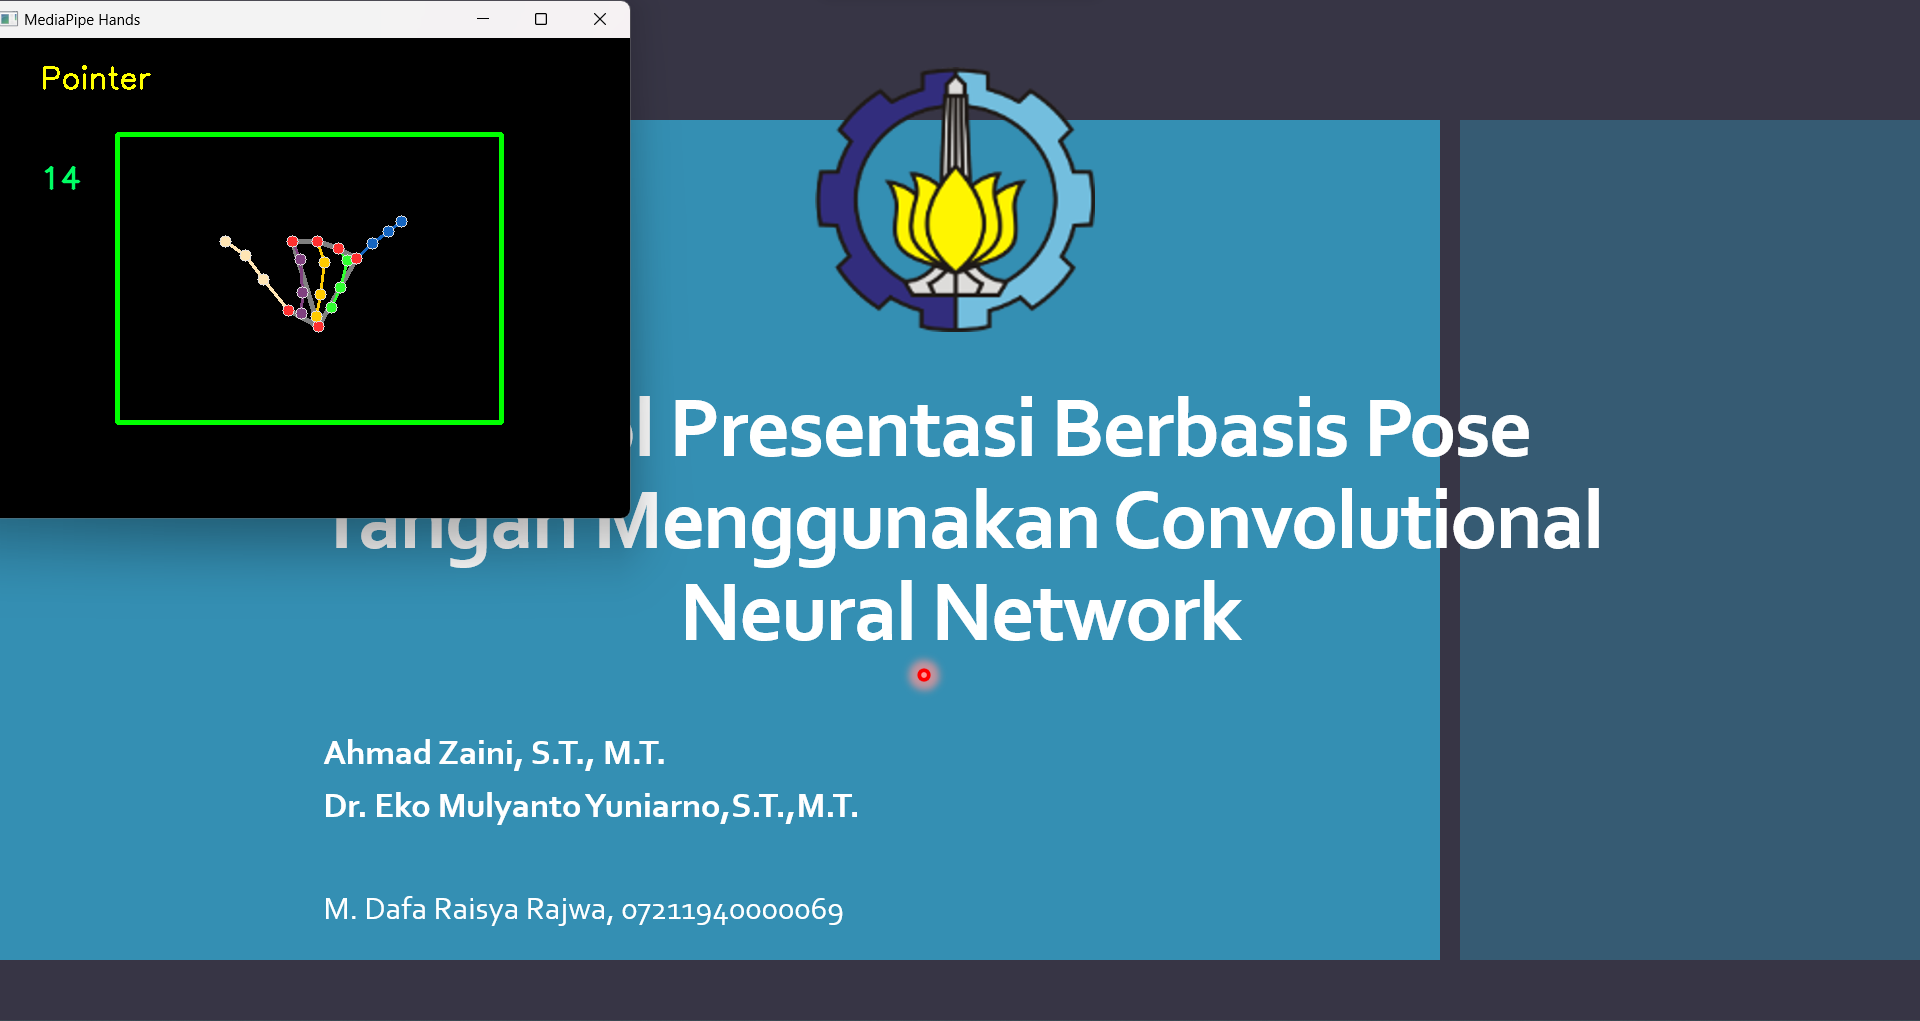
\includegraphics[scale=0.38]{gambar/hasil-kontrol-PPT.png}
% %   \caption{Kontrol Pointer}
% %   \label{fig:Kontrol Pointer}
% % \end{figure}

% \subsection{Kontrol \emph{Pen}}
% \label{subsec:Kontrol Pen}

% Dalam penerapan fungsi \emph{pen} penentuan titik koordinatnya sama persis dengan yang fungsi \emph{pointer} yang dijelaskan pada Subbab \ref{subsec:Kontrol Pointer}. Pembedanya adalah pada kondisi untuk menggambarnya. Pada kontrol ini saat posisi pose \emph{pen} terdeteksi, program dibuat untuk berpindah \emph{state} kedalam mode menggambar.

% Perubahan \emph{state} yang dilakukan memiliki tujuan tertentu. Pertama, dapat menghindari perubahan hasil deteksi ketika sedang menggerakkan tangan ketika menggambar. Selain itu, saat berubah \emph{state} proses prediksi model untuk klasifikasi juga tidak dijalankan. Sehingga saat sedang menggambar diharapkan tidak terjadi proses komputasi yang tidak perlu dan bisa menurunkan \emph{frame rate}.

% Pada \emph{state pen} ini mengaktifkan fitur \emph{pen} dan menggerakkan \emph{cursor}, namun tidak menekan tombol klik. Penekanan tombol klik baru dilakukan ketika bagian ujung jempol dihubungkan dengan jari tengah. mekanisme tersebut dibuat agar penggunaan fitur \emph{pen} terasa lebih mudah seperti menggunakan \emph{mouse}. Cara kerjanya adalah dengan mengukur jarak antara titik ujung jempol dengan bagian dari jari tengah. Tepatnya pada titik \emph{landmark} ke-10 dan ke-4 (Detail letak titik ini dapat dilihat pada Tabel \ref{tb:keterangansetiaptitiklandmark}). Jika jaraknya diangka lebih kecil dari 0,05 maka program mengirimkan input untuk menekan klik kiri pada \emph{mouse} dan jika tidak maka penekanan klik ini akan dilepaskan.

% \subsection{Kontrol \emph{Zoom In}}
% \label{subsec:Kontrol Zoom In}

% Kontrol zoom pada dasarnya sama dengan pen, yang membedakan pada kondisi \emph{trigger} fungsi zoom. Pada kontrol ini yang menjadi acuan adalah jarak antara ujung jempol dengan ujung telunjuk. Lebih tepatnya titik \emph{landmark} ke-8 dan ke-4. Jika jaraknya masih terhitung menempel maka fungsi zoom belum dijalankan. Namun, jika jaraknya mulai menjauh baru menjalankan fungsi zoom. Besarnya zoom yang dilakukan adalah sebesar 50\%. 

% \subsection{Kontrol \emph{Erase}}
% \label{subsec:Kontrol Erase}
% Kontrol pada \emph{erase} lebih sederhana dibandingkan dengan fungsi-fungsi sebelumnya. Jika hasil prediksi pose menghasilkan kelas \emph{erase}, maka program menjalankan fungsi \emph{erase} melalui \emph{library pyautogui}. Perlu diketahui bahwa fungsi \emph{erase} disini untuk menghapus coretan \emph{pen}. Penghapusan yang dilakukan langsung membersihkan seluruh coretan dalam satu layar sekaligus.